%%
%% This is file `hustreport-zh-example.tex',
%% generated with the docstrip utility.
%%
%% The original source files were:
%%
%% hustreport.dtx  (with options: `example-zh')
%% 
%% This is a generated file.
%% 
%% Copyright (C) 2013-2014 by Xu Cheng <xucheng@me.com>
%%               2014-2016 by hust-latex <https://github.com/hust-latex>
%% 
%% This work may be distributed and/or modified under the
%% conditions of the LaTeX Project Public License, either version 1.3
%% of this license or (at your option) any later version.
%% The latest version of this license is in
%%   http://www.latex-project.org/lppl.txt
%% and version 1.3 or later is part of all distributions of LaTeX
%% version 2005/12/01 or later.
%% 
%% This work has the LPPL maintenance status `maintained'.
%% 
%% The Current Maintainer of this work is hust-latex Organization.
%% 
%% This work consists of the files hustreport.dtx,
%% hustreport.ins and the derived file hustreport.cls
%% along with its document and example files.
%% 
%% \CharacterTable
%% {Upper-case    \A\B\C\D\E\F\G\H\I\J\K\L\M\N\O\P\Q\R\S\T\U\V\W\X\Y\Z
%%  Lower-case    \a\b\c\d\e\f\g\h\i\j\k\l\m\n\o\p\q\r\s\t\u\v\w\x\y\z
%%  Digits        \0\1\2\3\4\5\6\7\8\9
%%  Exclamation   \!     Double quote  \"     Hash (number) \#
%%  Dollar        \$     Percent       \%     Ampersand     \&
%%  Acute accent  \'     Left paren    \(     Right paren   \)
%%  Asterisk      \*     Plus          \+     Comma         \,
%%  Minus         \-     Point         \.     Solidus       \/
%%  Colon         \:     Semicolon     \;     Less than     \<
%%  Equals        \=     Greater than  \>     Question mark \?
%%  Commercial at \@     Left bracket  \[     Backslash     \\
%%  Right bracket \]     Circumflex    \^     Underscore    \_
%%  Grave accent  \`     Left brace    \{     Vertical bar  \|
%%  Right brace   \}     Tilde         \~}
\documentclass[format=draft,language=chinese,category=academic-report]{hustreport}

\stuno{1111}
\title{基于前馈神经网络的分类任务设计}
\author{thezmmm}
\major{数据科学与大数据技术}
\class{000}
\advisor{杨卫}

\begin{document}

\frontmatter
\maketitle
\tableofcontents
\mainmatter

\chapter{实验要求}
\begin{enumerate}
\item 实验目标:

设计一个卷积神经网络并使用ResNet模块,在MNIST数据集上实现10分类手写数字识别。实验报告将包括以下内容:神经网络架构、每轮mini-batch训练后模型在训练集和测试集上的损失、最终的训练集和测试集准确率、不同设计变化导致的网络性能差异以及相应的实验分析。

\item 数据集描述:

本实验使用的数据集是MNIST(Modified National Institute of Standards and Technology)手写数字数据集。该数据集是一个广泛应用于机器学习和计算机视觉领域的经典数据集,用于手写数字识别任务。

数据集由来自250位不同人手写的60,000个训练样本和10,000个测试样本组成。每个样本都是一个28x28像素的灰度图像,表示了手写的0到9之间的单个数字。

数据集中的图像已经经过预处理,像素值被归一化到0到1之间的范围。这意味着每个像素的灰度值都在0到255之间,通过除以255,将像素值缩放到0到1之间,使得处理过程更加稳定。

在实验中,数据集被划分为训练集和测试集,其中训练集用于模型的训练和参数优化,测试集用于评估模型的性能和泛化能力。

\item ResNet网络:

ResNet(Residual Neural Network)是一种深度卷积神经网络结构,由Kaiming He等人在2015年提出。它被设计用于解决深层神经网络训练过程中的梯度消失和梯度爆炸问题,使得可以训练更深的网络,同时提高了模型的性能。

ResNet的核心思想是引入了残差连接(residual connections),允许网络通过跨层直接的捷径连接来传递信息。传统的深层神经网络在进行前向传播时,输入数据通过一系列的卷积层和非线性激活函数后,逐渐转化为高级特征。然而,随着网络层数的增加,深层网络往往会出现梯度消失或梯度爆炸的问题,导致模型难以训练。

ResNet通过在网络中引入残差模块来解决这个问题。残差模块的基本组成是一个跨层的残差块(residual block),其中包含了跳跃连接(skip connection)和恒等映射(identity mapping)。

在传统的残差块中,输入数据经过一系列的卷积层和非线性激活函数后,与原始输入进行元素级的相加操作。这样做的好处是,在反向传播时可以通过梯度传递直接更新原始输入,避免了梯度的消失和爆炸。

此外,为了保持特征维度的一致性,对于跨层的连接,ResNet使用了一个额外的1x1卷积层来调整通道数,使得输入和输出的特征图具有相同的维度。

ResNet的架构可以根据任务的复杂度和深度进行调整。通常,ResNet由多个残差块组成,其中每个残差块可以包含两个或三个卷积层。较深的ResNet模型还会引入池化层和全连接层。

通过引入残差连接,ResNet在训练深层网络时具有以下优势:
\begin{itemize}
\item 解决了梯度消失和梯度爆炸问题,使得可以训练更深的网络。
\item 通过跨层的信息传递,提高了特征的流动性,有助于学习更准确的特征表示。
\item 引入了更少的参数,减少了模型的复杂性,降低了过拟合的风险。
\item 对于浅层网络,ResNet可以退化为普通的卷积神经网络。
\end{itemize}
\end{enumerate}
\chapter{实验内容}
\section{残差模块}
\begin{lstlisting}
def resnet_block(x, filters, downsample=False):
    identity = x

    # 第一个卷积层
    x = layers.Conv2D(filters, kernel_size=(3, 3), strides=(1 if not downsample else 2, 1 if not downsample else 2), padding='same')(x)
    x = layers.BatchNormalization()(x)
    x = layers.Activation(activation_function)(x)

    # 第二个卷积层
    x = layers.Conv2D(filters, kernel_size=(3, 3), strides=(1, 1), padding='same')(x)
    x = layers.BatchNormalization()(x)

    # 如果下采样,使用1x1卷积进行维度匹配
    if downsample:
        identity = layers.Conv2D(filters, kernel_size=(1, 1), strides=(2, 2), padding='same')(identity)
        identity = layers.BatchNormalization()(identity)

    # 残差连接
    x = layers.Add()([x, identity])
    x = layers.Activation(activation_function)(x)

    return x
\end{lstlisting}
该残差块的输入为x,filters参数表示卷积层的滤波器数量,downsample参数用于指示是否进行下采样。

首先,将输入x保存在变量identity中,作为后续的跳跃连接(skip connection)。

然后,进行第一个卷积层操作。使用大小为3x3的卷积核,步长为1(如果未进行下采样)或2(如果进行下采样),填充方式为"same"(保持输入和输出的特征图大小相同)。卷积操作后,将通过批归一化(Batch Normalization)层进行规范化,以提高模型的稳定性和训练速度。最后,通过激活函数(activation\_function)对特征图进行激活。

接下来,进行第二个卷积层操作。同样使用大小为3x3的卷积核,步长为1,填充方式为"same"。卷积操作后,再次通过批归一化层进行规范化。

如果进行下采样,即downsample为True,那么需要对identity进行维度匹配。这里使用了一个1x1的卷积层,步长为2,目的是将identity的特征图大小与卷积层的输出特征图大小保持一致。同样,经过卷积操作后,通过批归一化层进行规范化。

最后,通过残差连接将第二个卷积层的输出x与identity相加。这里使用了Add()层来实现元素级相加。通过残差连接,网络可以直接传递原始输入的信息,有助于避免梯度消失和梯度爆炸的问题。相加操作后,再通过激活函数对结果进行激活。

整个残差块的输出为x,表示经过残差连接后的特征图。这样的残差块可以在ResNet网络中被重复堆叠,以构建深层模型,并提高模型的性能和训练效果。

此外,代码中使用了activation\_function作为激活函数的占位符。在实际实验过程中,其被替换为具体的激活函数,例如ReLU、Leaky ReLU等。
\section{神经网络模型}
\begin{lstlisting}
def build_model():
    inputs = tf.keras.Input(shape=(28, 28, 1))

    # 第一个卷积层
    x = layers.Conv2D(64, kernel_size=(7, 7), strides=(2, 2), padding='same')(inputs)
    x = layers.BatchNormalization()(x)
    x = layers.Activation(activation_function)(x)
    x = layers.MaxPooling2D(pool_size=(3, 3), strides=(2, 2), padding='same')(x)

    # 使用ResNet模块构建网络
    x = resnet_block(x, filters=64)
    x = resnet_block(x, filters=64)
    x = resnet_block(x, filters=64)

    x = layers.GlobalAveragePooling2D()(x)

    # 全连接层
    x = layers.Dense(64, activation=activation_function)(x)
    outputs = layers.Dense(10, activation='softmax')(x)

    model = tf.keras.Model(inputs=inputs, outputs=outputs)
    return model

\end{lstlisting}
该神经网络的输入是一个形状为(28, 28, 1)的图像。

首先,通过tf.keras.Input()函数创建了一个输入层,用于接收输入数据。

接下来是第一个卷积层。使用了64个大小为7x7的卷积核,步长为2,填充方式为"same"。卷积操作后,通过批归一化层进行规范化,然后通过激活函数进行激活。在激活后,进行了大小为3x3的最大池化操作,步长为2,填充方式为"same"。最大池化操作可以降低特征图的尺寸,并提取出主要的特征。

然后,使用了三个ResNet模块(resnet\_block)构建了网络。每个模块都使用了64个滤波器。这些模块通过残差连接,提供了跨层的信息传递和特征重用。这样的设计有助于训练深层网络,并提高模型的性能。

在ResNet模块之后,使用了一个全局平均池化层(GlobalAveragePooling2D)。该层对每个特征图进行平均池化操作,将特征图的空间维度降为1,保留了每个特征通道的平均值。这有助于减少参数数量,并提取出整体的图像特征。

最后,通过一个全连接层(Dense)进行特征映射,使用64个神经元和指定的激活函数。然后,使用另一个全连接层生成输出,使用10个神经元和softmax激活函数,用于多类别分类任务。

最终,使用tf.keras.Model()函数将输入层和输出层组合成一个模型,并返回该模型。

\begin{figure}[htbp]
\centering
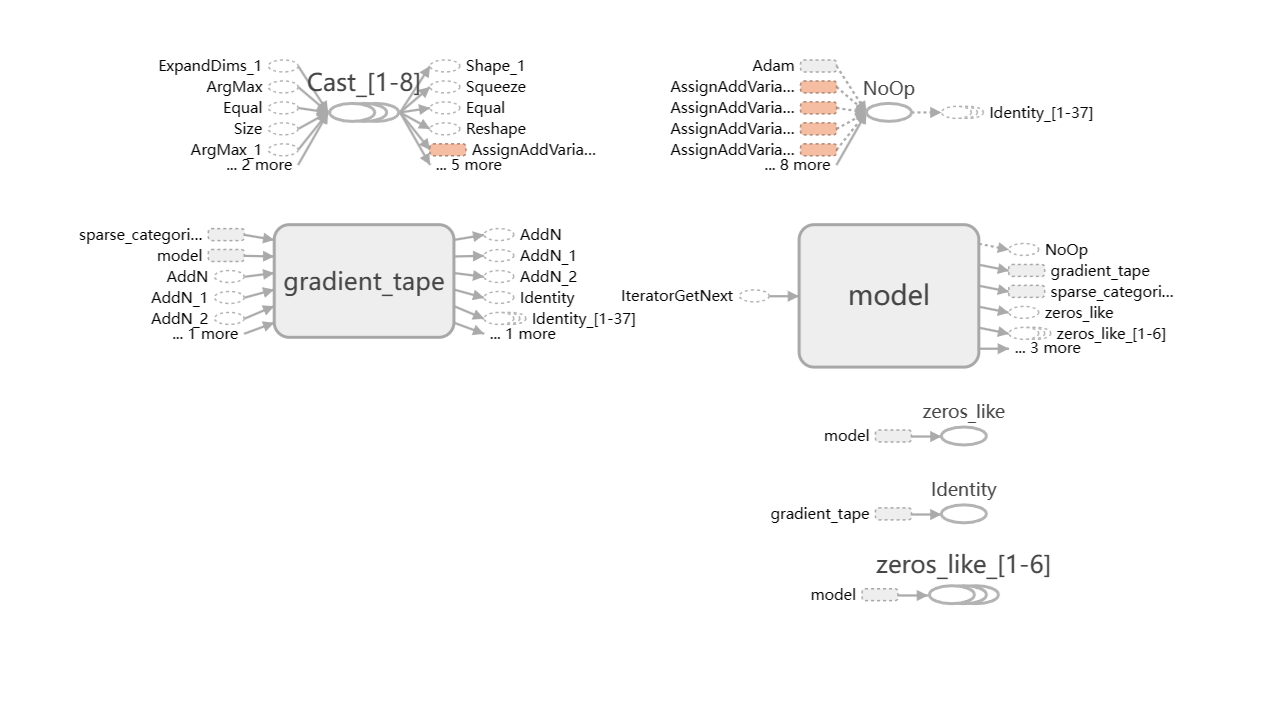
\includegraphics[scale=0.4]{img/batchsize_64_optimizer_Adam_loss_sparse_categorical_crossentropy_activation_ReLU_lr_0.001_train1.png}
\caption{神经网络架构图1}
\end{figure}

\begin{figure}[htbp]
\centering
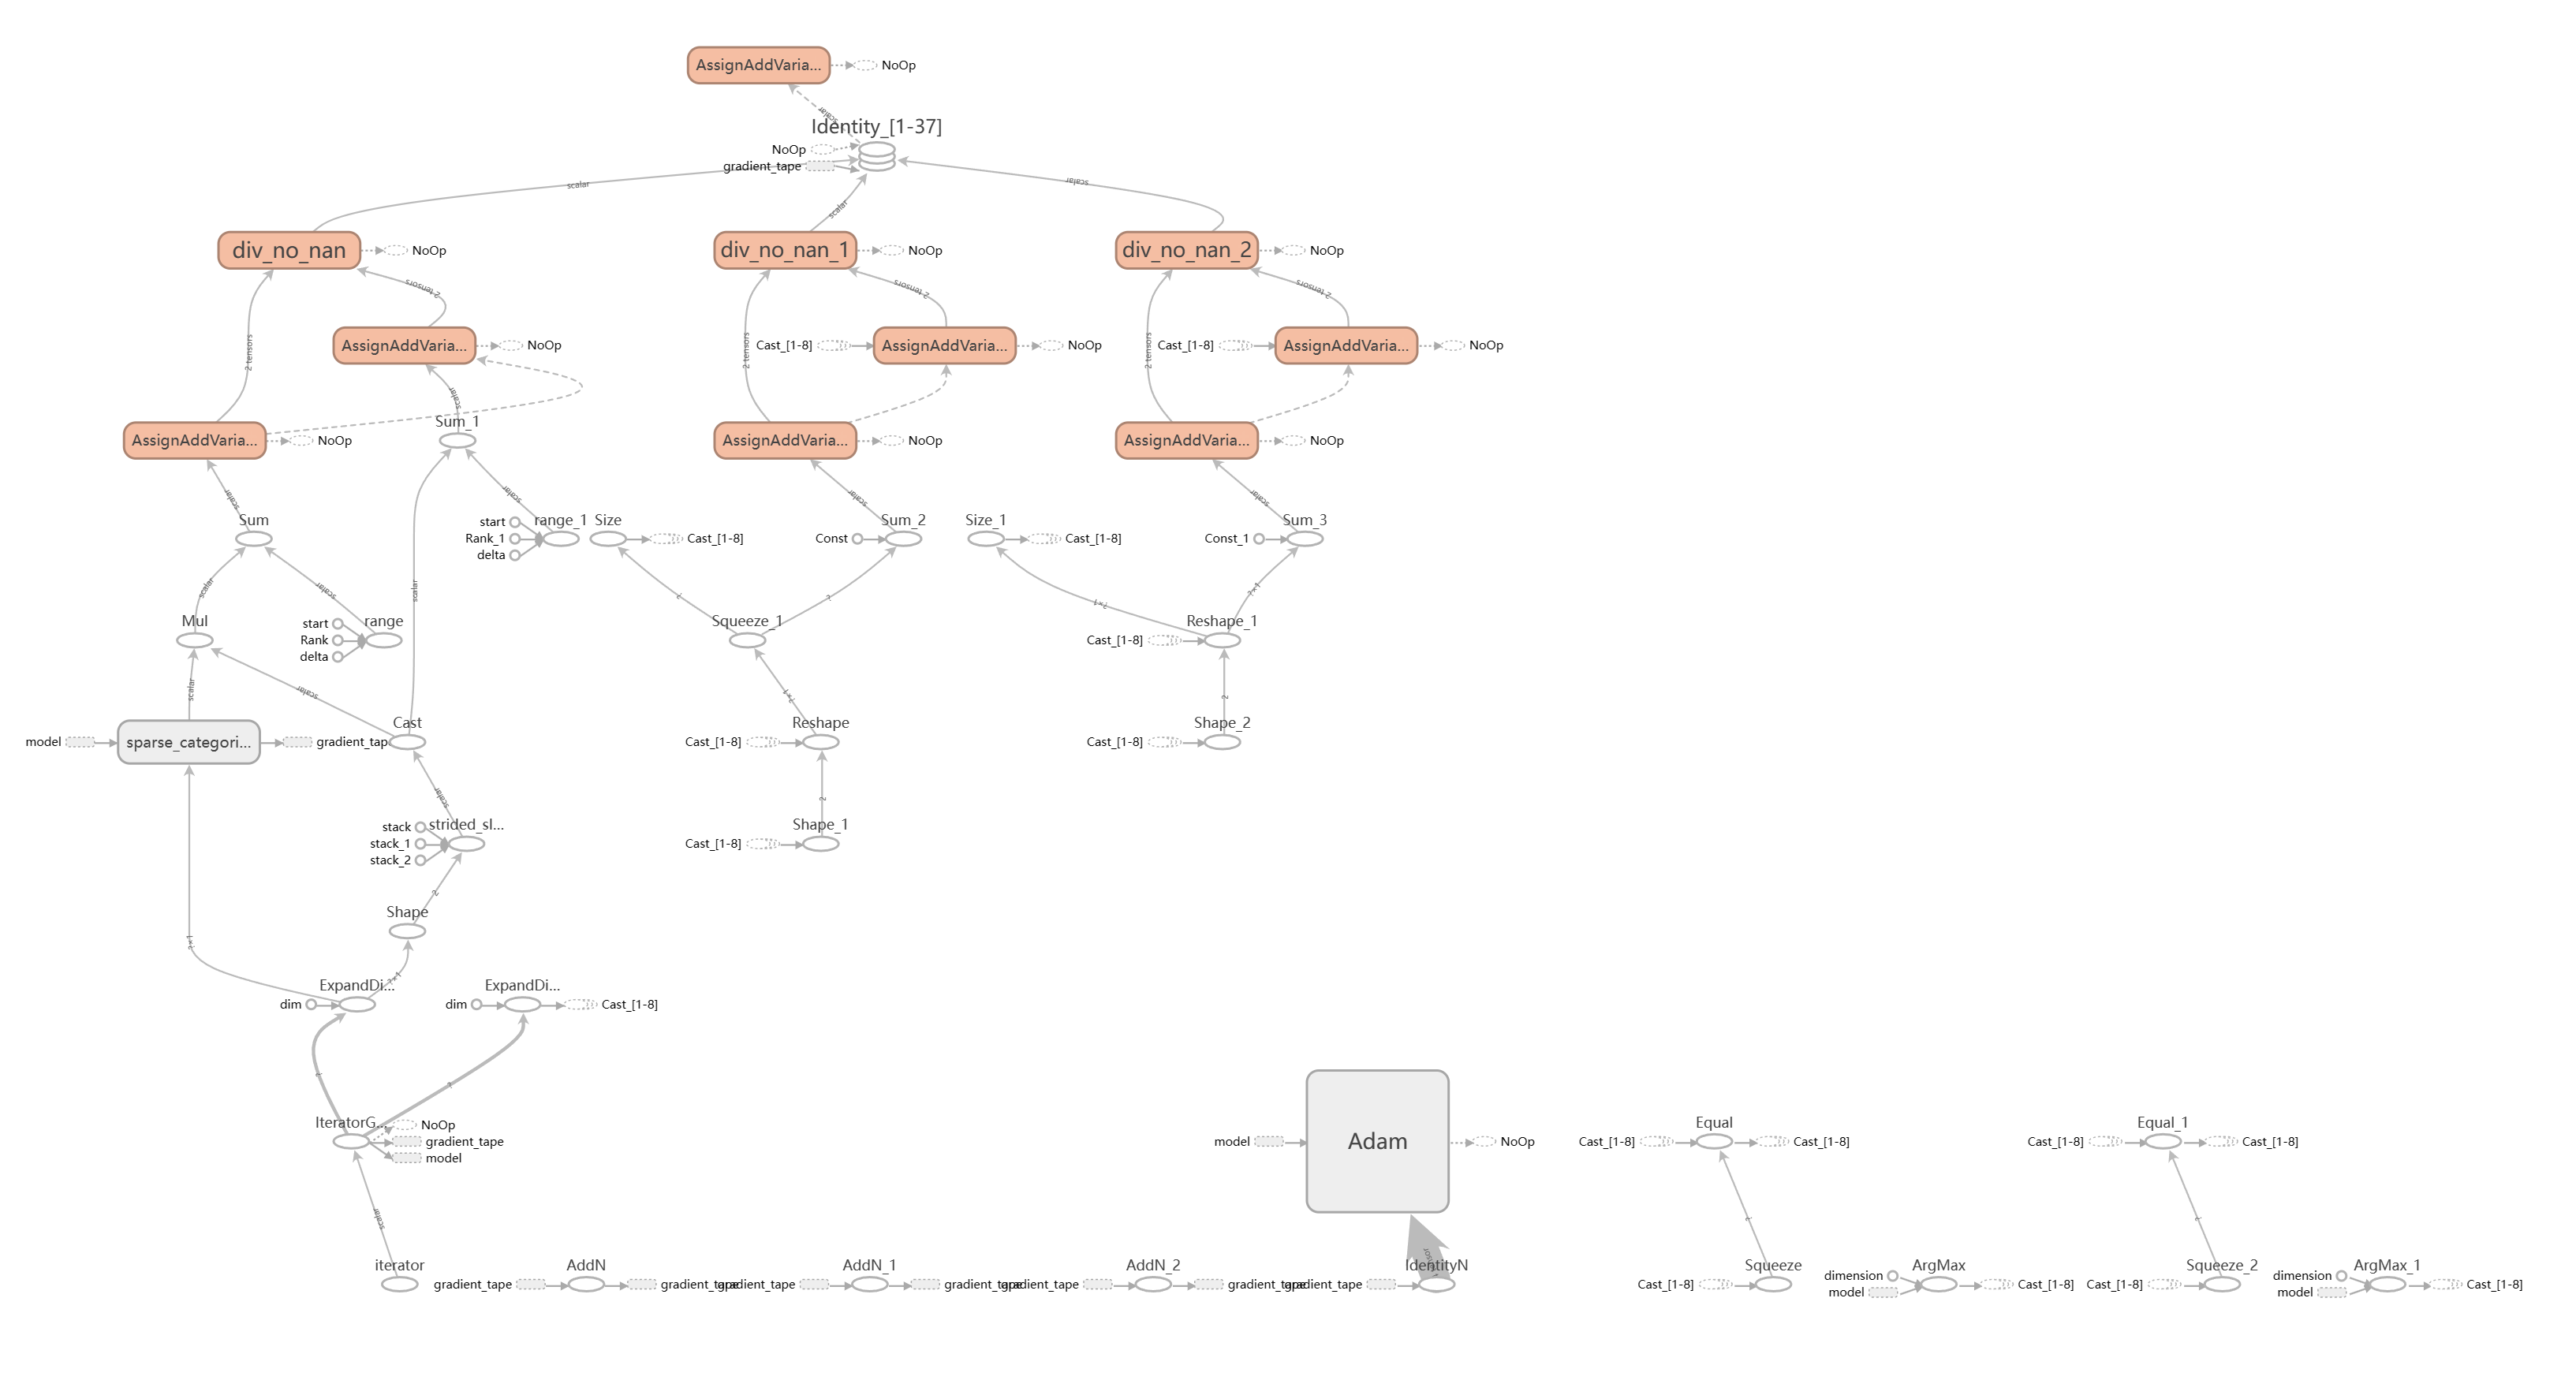
\includegraphics[scale=0.2]{img/batchsize_64_optimizer_Adam_loss_sparse_categorical_crossentropy_activation_ReLU_lr_0.001_train2.png}
\caption{神经网络架构图2}
\end{figure}

\section{网络参数}
在实验中,测试了不同的激活函数、优化器、学习率和批量大小对网络的影响。下面是这些参数的详细说明:
\subsection{激活函数 (Activation Function)}
在神经网络中,激活函数被用于引入非线性特性,以增加神经网络的表示能力。在实验中,我使用了不同的激活函数进行测试,如ReLU、Sigmoid、Tanh等。不同的激活函数会对网络的学习能力和收敛速度产生不同的影响。
\subsection{优化器 (Optimizer):}
优化器是用来更新神经网络的权重和偏置的算法。实验中,我使用了几个比较常见的优化器,如随机梯度下降(SGD)、Adam、RMSprop等。不同的优化器具有不同的更新策略和超参数,可以对网络的训练效果产生显著影响。
\subsection{学习率 (Learning Rate):}
学习率决定了每次权重更新的步长大小。在实验中,我测试了不同的学习率值,以观察其对网络性能的影响。学习率过高可能导致训练不稳定或无法收敛,学习率过低可能导致训练速度慢或陷入局部最优。选择合适的学习率是一项关键任务,通常需要通过实验和调优来确定最佳值。
\subsection{批量大小 (Batch Size):}
批量大小确定了每次迭代中用于更新参数的样本数量。在实验中,我测试了不同的批量大小值,以观察其对网络训练的影响。较大的批量可以加快训练速度,但可能导致内存消耗较大;较小的批量可以提供更好的梯度估计,但训练速度较慢。选择合适的批量大小需要权衡训练速度和模型性能。

\section{自定义指标}
\begin{lstlisting}
# 自定义指标,查看每个类别的准确度
class PerClassAccuracy(tf.keras.callbacks.Callback):
    def __init__(self, validation_data):
        super(PerClassAccuracy, self).__init__()
        self.validation_data = validation_data

    def on_epoch_end(self, epoch, logs=None):
        # 预测验证集数据
        predictions = self.model.predict(self.validation_data[0])
        predicted_labels = tf.argmax(predictions, axis=1)

        # 计算每个类别的准确度
        num_classes = len(tf.unique(self.validation_data[1])[0])
        class_accuracy = []
        for class_id in range(num_classes):
            class_indices = tf.where(tf.equal(self.validation_data[1], class_id))
            class_labels = tf.gather(self.validation_data[1], class_indices)
            class_predictions = tf.gather(predicted_labels, class_indices)

            # 将class_labels和class_predictions转换为int64类型
            class_labels = tf.cast(class_labels, tf.int64)
            class_predictions = tf.cast(class_predictions, tf.int64)

            accuracy = tf.reduce_mean(tf.cast(tf.equal(class_labels, class_predictions), tf.float32))
            class_accuracy.append(accuracy)

        # 将每个类别的准确度添加到日志中
        for class_id, accuracy in enumerate(class_accuracy):
            logs[f'val_accuracy_class_{class_id}'] = accuracy
\end{lstlisting}
这是一个自定义指标类PerClassAccuracy,它可以在每个类别上计算并打印分类准确度。

在初始化方法中,该类接收一个验证数据(validation\_data)作为参数。在每个epoch结束时,on\_epoch\_end方法会被调用。

在on\_epoch\_end方法中,首先使用模型对验证数据(validation\_data)进行预测,得到预测结果(predictions)。然后,使用tf.argmax函数找到每个样本的预测类别,即预测概率最大的类别。

接下来,通过计算唯一类别的数量,确定了num\_classes。

然后,对于每个类别,通过使用tf.where函数找到验证数据中属于该类别的样本索引(class\_indices)。然后,使用tf.gather函数从验证数据中获取属于该类别的标签(class\_labels)和预测结果(class\_predictions)。这样就得到了该类别的标签和预测结果。

接着,将class\_labels和class\_predictions转换为int64类型,以便进行后续计算。

接下来,通过计算tf.reduce\_mean函数对预测结果和标签进行比较,得到该类别的准确度(accuracy)。这里使用tf.equal函数比较两个张量的元素是否相等,然后使用tf.cast函数将布尔型的结果转换为float32类型。

最后,将每个类别的准确度添加到logs字典中,使用类别的索引(class\_id)作为键,并以val\_accuracy\_class\_作为前缀。这样,在训练过程中,每个epoch结束后,这些准确度就会作为日志打印出来。

通过使用这个自定义指标,可以在训练过程中实时监控每个类别的分类准确度,以更好地了解模型在不同类别上的表现。
\chapter{实验结果}
\section{激活函数的影响}
根据实验结果,可以对三种不同的激活函数(ReLU、Sigmoid和Tanh)对网络性能的影响进行分析。下面是对每个激活函数的影响进行详细分析:
\begin{figure}[htbp]
\centering
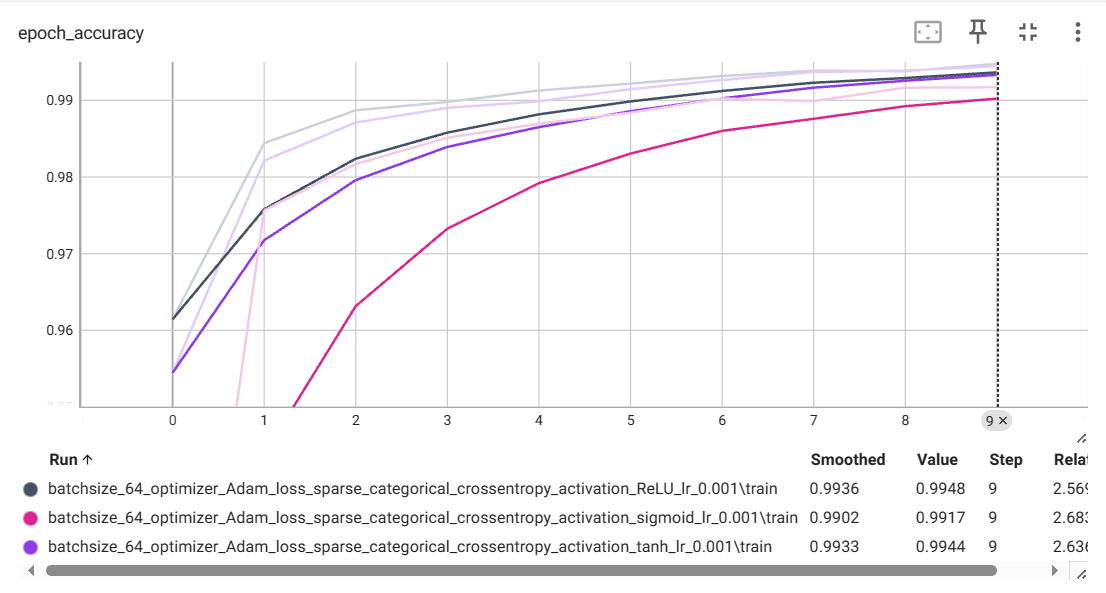
\includegraphics[scale=0.4]{img/epoch_accuracy_activation_train.png}
\caption{不同激活函数的准确率}
\end{figure}
\begin{figure}[htbp]
\centering
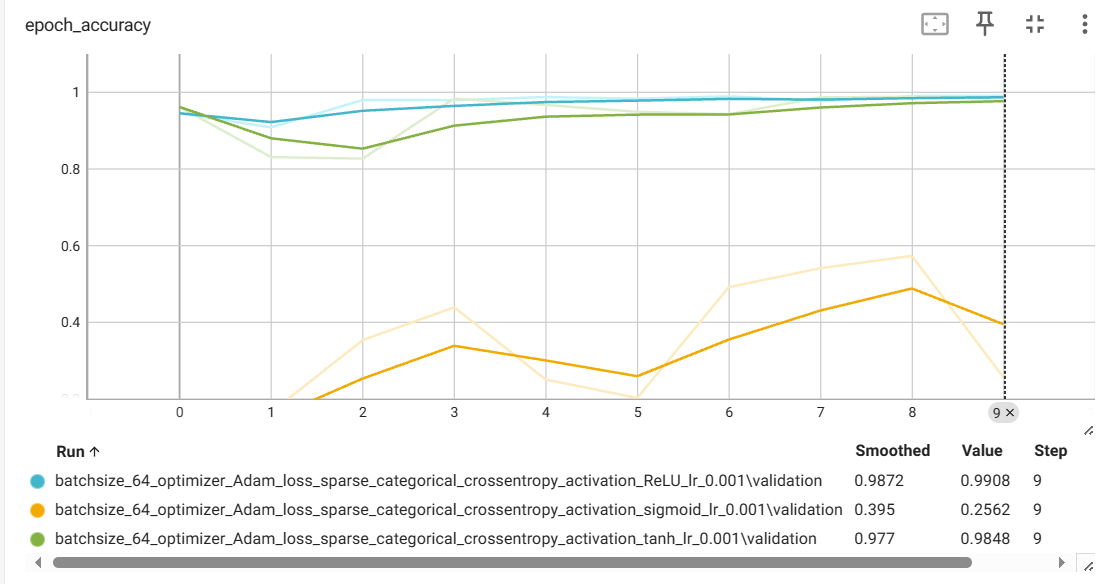
\includegraphics[scale=0.4]{img/epoch_accuracy_activation_val.png}
\caption{不同激活函数在验证集上的准确率}
\end{figure}
\begin{enumerate}
\item ReLU激活函数:

在训练集上的准确度逐渐提高,从初始值0.9614增加到最终值0.9947。

在验证集上的准确度有一定的波动,但整体上保持在较高水平,从初始值0.9454增加到最终值0.9908。

原因:Relu激活函数在正值区间具有线性特性,能够很好地捕捉到正向信号。这有助于提高网络的表达能力和非线性建模能力,从而在训练集和验证集上获得较高的准确度。
\item Sigmoid激活函数:

在训练集上的准确度也有所提高,从初始值0.8908增加到最终值0.9917。

在验证集上的准确度出现了较大的波动,从初始值0.1218增加到最高值0.5733,然后回落到较低的值。

原因:Sigmoid激活函数的输出范围在(0, 1)之间,可以用作二分类问题的输出。然而,对于多类别分类问题,Sigmoid函数的输出并没有明确的类别边界,这可能导致模型在验证集上的性能波动较大。
\item Tanh激活函数:

在训练集上的准确度逐渐提高,从初始值0.9545增加到最终值0.9944。

在验证集上的准确度有一定的波动,但整体上保持在较高水平,从初始值0.9619增加到最终值0.9848。

原因:Tanh激活函数在负值区间和正值区间都具有非线性特性,可以更好地处理正负信号。这有助于提高模型的拟合能力和分类性能,从而在训练集和验证集上获得较高的准确度。
\end{enumerate}
综上所述,Relu和Tanh激活函数在训练集和验证集上都表现出较好的性能,而Sigmoid激活函数在验证集上的性能不稳定。这可能是由于Sigmoid函数的输出范围和特性对多类别分类问题的适应性较差。因此,在多类别分类任务中,使用Relu或Tanh激活函数能够获得更好的性能。
\section{优化器的影响}
根据实验结果,可以对三种不同的优化器(Adam、SGD和RMSprop)对网络性能的影响进行分析。下面是对每个优化器的影响进行详细分析:
\begin{figure}[htbp]
\centering
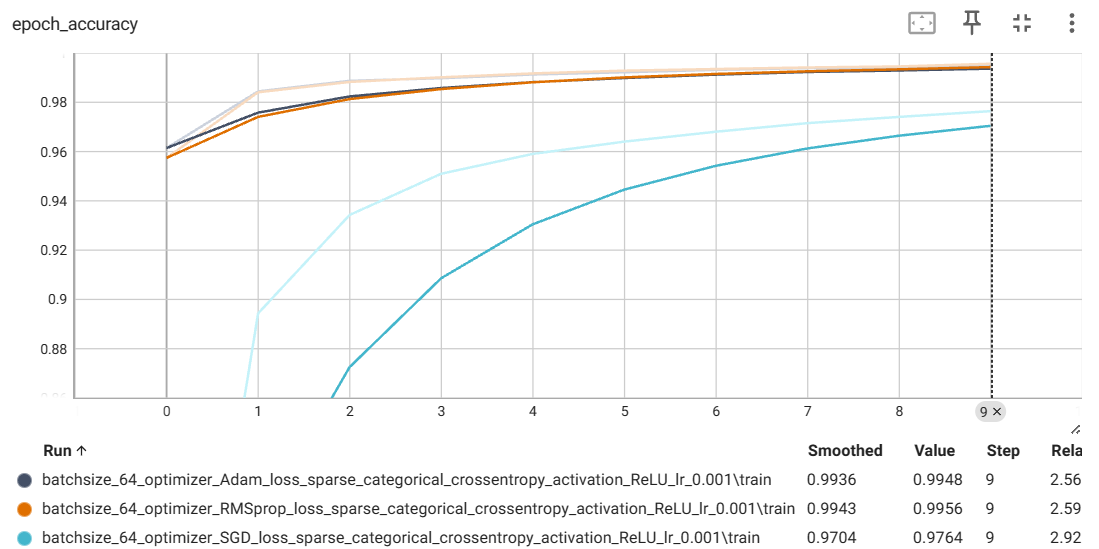
\includegraphics[scale=0.4]{img/epoch_accuracy_optimizer_train.png}
\caption{不同优化器的准确率}
\end{figure}
\begin{figure}[htbp]
\centering
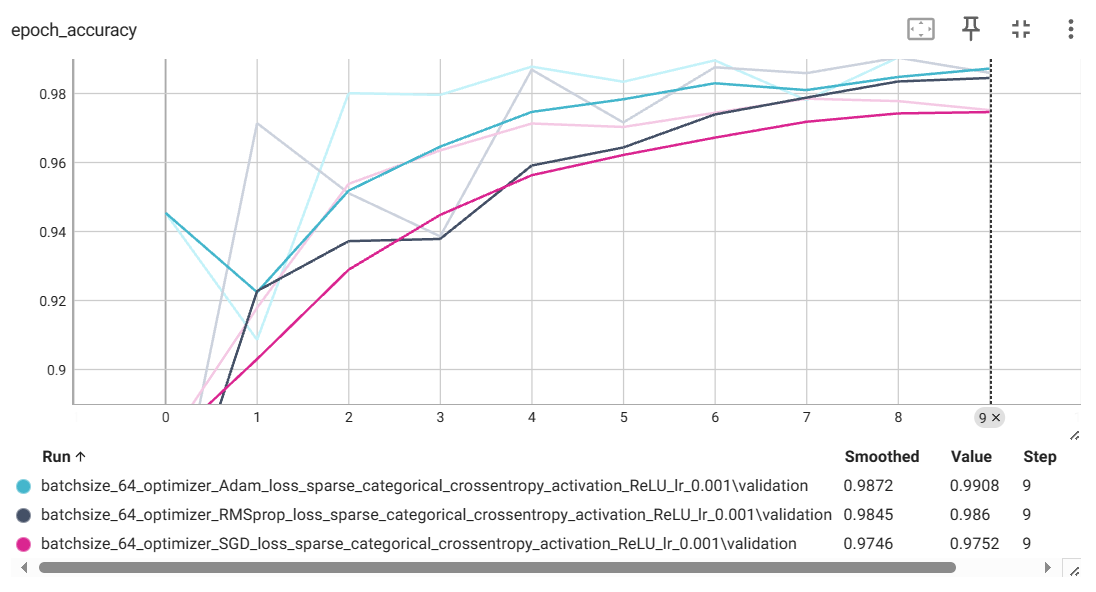
\includegraphics[scale=0.4]{img/epoch_accuracy_optimizer_val.png}
\caption{不同优化器在验证集上的准确率}
\end{figure}
\begin{enumerate}
\item Adam优化器:

在训练集上的准确度逐渐提高,从初始值0.9614增加到最终值0.9947。

在验证集上的准确度有一定的波动,但整体上保持在较高水平,从初始值0.9454增加到最终值0.9908。

原因:Adam优化器结合了动量优化和自适应学习率的特性,能够快速收敛并且适应不同的参数更新速度。它在训练过程中能够更好地平衡梯度的方向和大小,从而提高网络的收敛性和泛化能力。
\item SGD优化器:

在训练集上的准确度也有所提高,从初始值0.6648增加到最终值0.9764。

在验证集上的准确度也有一定的提高,从初始值0.8782增加到最终值0.9752。

原因:SGD优化器是一种基本的优化算法,通过计算梯度并更新参数来最小化损失函数。尽管SGD可以收敛到局部最优解,但由于其对参数更新的简单性,可能会陷入局部最优或平原区域。然而,在某些情况下,SGD可能会在训练集和验证集上获得相对较好的性能。
\item RMSprop优化器:

在训练集上的准确度逐渐提高,从初始值0.9574增加到最终值0.9956。

在验证集上的准确度有一定的波动,但整体上保持在较高水平,从初始值0.8416增加到最终值0.9860。

原因:RMSprop优化器在计算梯度时考虑了梯度的平方平均值,根据平均梯度的大小自适应地调整学习率。这有助于处理不同参数的学习速度差异,从而提高网络的收敛速度和稳定性。
\end{enumerate}
综上所述,Adam和RMSprop优化器在训练集和验证集上表现出较好的性能,能够更好地平衡梯度更新和学习率调整。SGD优化器在性能方面略逊一筹,但在某些情况下仍然可以获得相对较好的结果。因此,在选择优化器时,优先考虑Adam和RMSprop来获得更好的网络性能。
\section{学习率的影响}
根据实验结果,可以对三种不同的学习率对网络性能的影响进行分析。下面是对学习率的影响进行详细分析:
\begin{figure}[htbp]
\centering
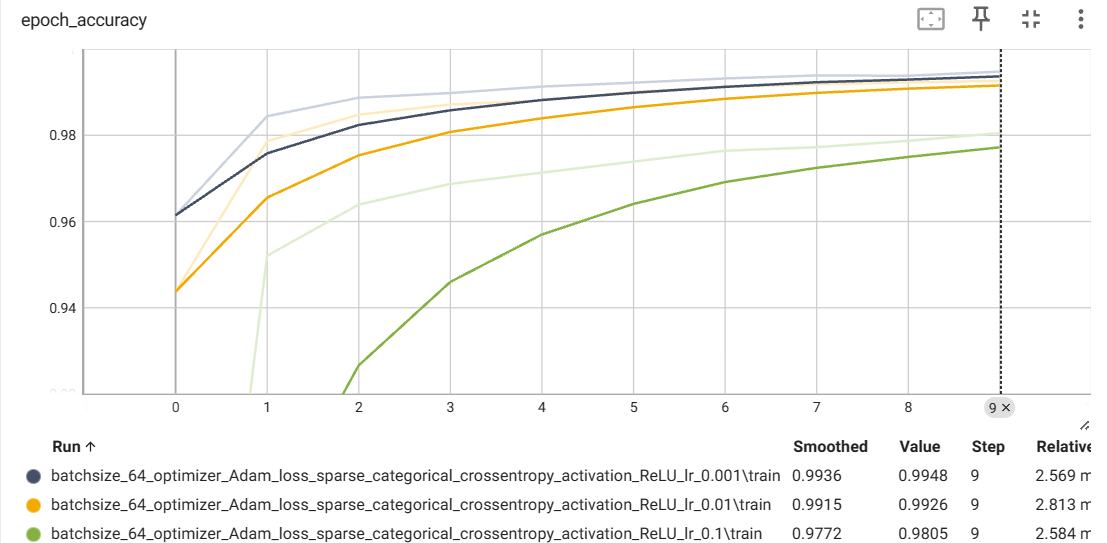
\includegraphics[scale=0.4]{img/epoch_accuracy_lr_train.png}
\caption{不同学习率的准确率}
\end{figure}
\begin{figure}[htbp]
\centering
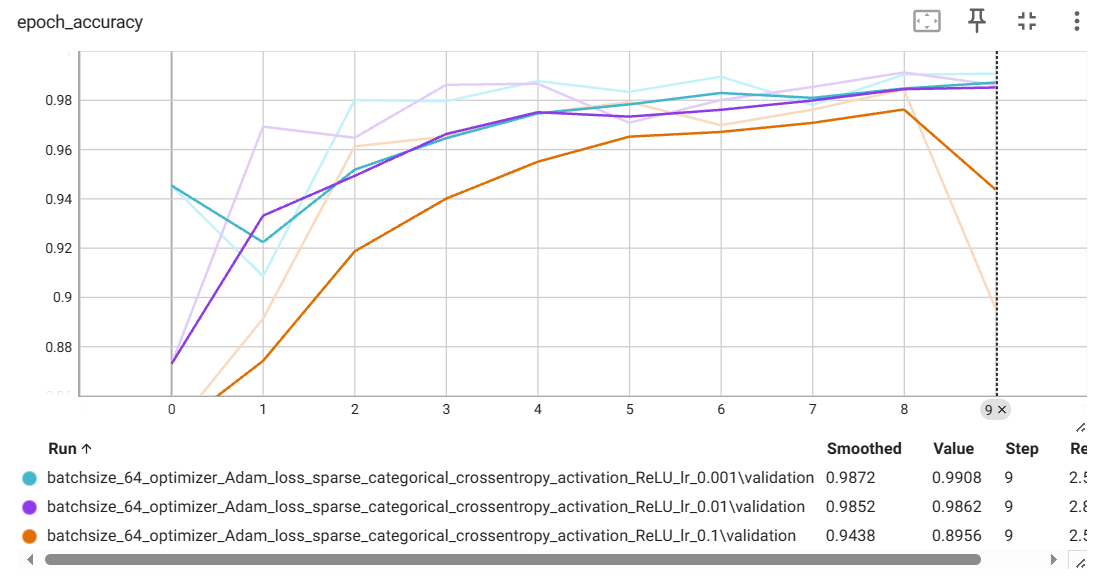
\includegraphics[scale=0.4]{img/epoch_accuracy_lr_val.png}
\caption{不同学习率在验证集上的准确率}
\end{figure}
\begin{enumerate}
\item 学习率为0.1:

在训练集上的准确度有所提高,从初始值0.7806增加到最终值0.9805。

在验证集上的准确度有一定的波动,从初始值0.8457增加到最终值0.8956。

原因:较高的学习率可能导致参数更新过大,使得网络在训练过程中难以收敛。在这种情况下,训练集的准确度可能会有所提高,但验证集的准确度可能会下降,因为网络过度拟合了训练数据。

\item 学习率为0.01:

在训练集上的准确度也有所提高,从初始值0.9437增加到最终值0.9926。

在验证集上的准确度整体上保持在较高水平,从初始值0.8730增加到最终值0.9862。

原因:适中的学习率可以使网络在训练过程中平稳地收敛。在这种情况下,网络能够在训练集和验证集上获得相对较好的性能,避免了过拟合和欠拟合的问题。

\item 学习率为0.001:

在训练集上的准确度逐渐提高,从初始值0.9614增加到最终值0.9947。

在验证集上的准确度有一定的波动,但整体上保持在较高水平,从初始值0.9454增加到最终值0.9908。

原因:较低的学习率可以使得参数更新更加稳定,有助于网络在训练过程中收敛到更好的解。在这种情况下,网络能够在训练集和验证集上获得相对较好的性能,但训练过程可能会较慢。
\end{enumerate}
综上所述,适当的学习率对网络性能至关重要。过高或过低的学习率都可能对网络的训练和泛化能力产生负面影响。在实践中,可以通过尝试不同的学习率并监控训练集和验证集的准确度来找到适合的学习率。通常情况下,较小的学习率能够带来更好的性能,但训练速度可能会较慢。
\section{批量大小的影响}
根据实验结果,可以对不同的批量大小对网络性能的影响进行分析。下面是对批量大小的影响进行详细分析:
\begin{figure}[htbp]
\centering
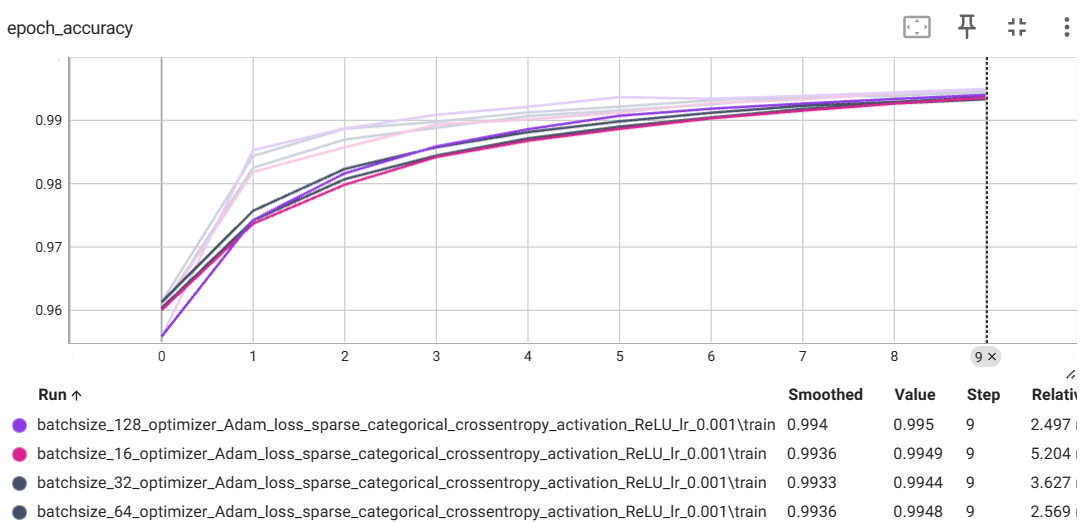
\includegraphics[scale=0.4]{img/epoch_accuracy_batchsize_train.png}
\caption{不同批量大小的准确率}
\end{figure}
\begin{figure}[htbp]
\centering
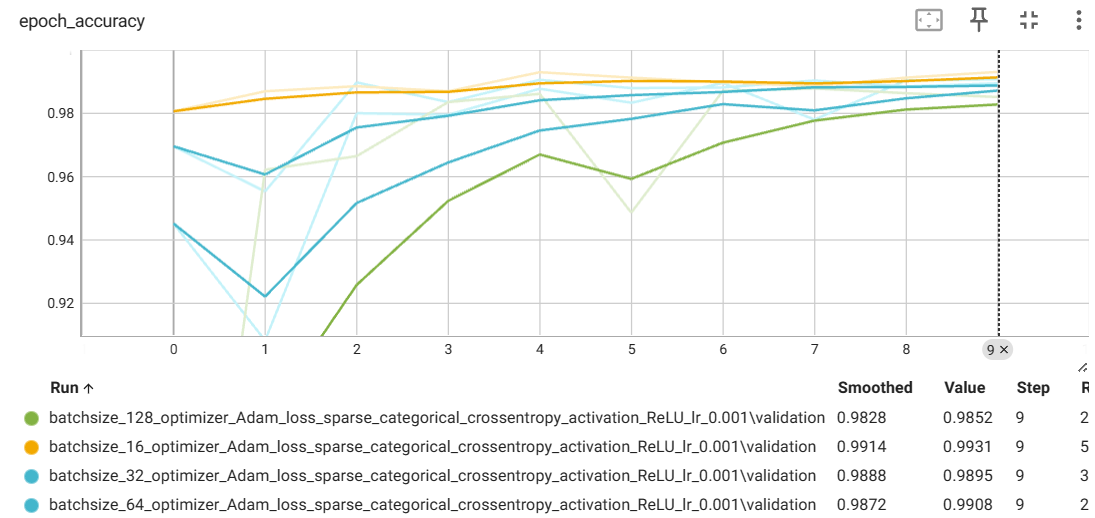
\includegraphics[scale=0.4]{img/epoch_accuracy_batchsize_val.png}
\caption{不同批量大小在验证集上的准确率}
\end{figure}
\begin{enumerate}
\item 批量大小为16:

在训练集上的准确度逐渐提高,从初始值0.9602增加到最终值0.9949。

在验证集上的准确度整体上保持在较高水平,从初始值0.9807增加到最终值0.9931。

原因:较小的批量大小可以提供更多的参数更新,使得网络能够更快地学习和收敛。这可能有助于网络在训练集和验证集上获得较好的性能。
\item 批量大小为32:

在训练集上的准确度逐渐提高,从初始值0.9605增加到最终值0.9944。

在验证集上的准确度有一定的波动,但整体上保持在较高水平,从初始值0.9697增加到最终值0.9895。

原因:适中的批量大小可以在一定程度上平衡参数更新的速度和稳定性。在这种情况下,网络能够在训练集和验证集上获得相对较好的性能,但可能略有波动。
\item 批量大小为64和128:

在训练集上的准确度逐渐提高,在初始值和最终值之间没有明显差异。

在验证集上的准确度有一定的波动,但整体上保持在较高水平。

原因:较大的批量大小可以减少参数更新的频率,有助于加速训练过程。然而,过大的批量大小可能会导致网络难以在验证集上泛化,因为每个批次中的样本差异较大。
\end{enumerate}
综上所述,选择适当的批量大小对网络性能非常重要。较小的批量大小可以加快训练速度并有助于网络收敛,但可能会导致训练过程中的波动。适中的批量大小通常能够在训练集和验证集上取得较好的性能。较大的批量大小可能加快训练速度,但可能降低验证集的性能。在实践中,可以尝试不同的批量大小并监控训练集和验证集的准确度来找到最佳的批量大小。
\chapter{总结}
本报告旨在研究基于卷积神经网络(CNN)的MNIST手写体数字识别任务。通过对实验结果的分析和探讨,得出以下结论:
\begin{enumerate}
\item 实验内容:

报告首先介绍了残差模块和神经网络模型,这些是构建卷积神经网络的基本组件。

接下来讨论了网络参数的选择,包括激活函数,优化器,学习率和批量大小等。

最后,报告介绍了自定义指标,用于评估模型性能。
\item 实验结果:

对不同激活函数的影响进行了分析,结果表明ReLU激活函数在MNIST任务中表现较好。

对优化器的影响进行了研究,Adam优化器在大多数情况下提供了良好的性能。

对学习率和批量大小的影响进行了探讨,适当的学习率和批量大小能够帮助网络获得最佳性能。 
\end{enumerate}

综上所述,通过基于卷积神经网络的MNIST手写体数字识别任务的研究,我们得出了一些关于激活函数、优化器、学习率和批量大小对网络性能的影响的结论。这些结果对于设计和优化卷积神经网络模型以实现准确的手写体数字识别具有重要意义。
\end{document}
\endinput
%%
%% End of file `hustreport-zh-example.tex'.
